\documentclass{beamer}
\usepackage{graphicx}
\usepackage{colortbl}
\usepackage{booktabs}
\usepackage{float}
\usepackage{subcaption}
\usepackage{multirow}
\usepackage{lmodern}


\usepackage[
authordate,
natbib,
backend=biber,
doi=false,
isbn=false,
url=false,
noibid=true
]{biblatex-chicago} % citation package

% natbib style commands
\renewcommand*{\nameyeardelim}{\addcomma\space}
% \newcommand*{\citep}{\parencite}
% \newcommand*{\citet}{\textcite}
\newcommand*{\citefoot}{\footcite}
\newcommand*{\citefull}{\fullcite}
\newcommand*{\citeno}{\nocite}
% \renewcommand*{\cite}{\textcite}

\addbibresource{reference.bib}%

\renewcommand\textbullet{\ensuremath{\bullet}}

\usepackage{silence}
\WarningFilter{biblatex}{Patching footnotes failed}


\usetheme{Singapore}
\setbeamercolor{section in head/foot}{bg=blue!50!red!30}
\title[Short title]{This is a long title}
\author[<%= Settings::LASTNAME %>]{<%= Settings::FIRSTNAME %> <%= Settings::MIDDLENAME %> <%= Settings::LASTNAME %>\inst{1}}


\institute{\inst{1}<%= Settings::DEPARTMENTNAME %> \\
<%= Settings::UNIVERISITYNAME %>}
\date{\today}
\graphicspath{ {figures/} }

\begin{document}

\begin{frame}
  \titlepage
\end{frame}


\section{Introduction}


\begin{frame}[t]\frametitle{Introduction}
    \begin{itemize}
      \item some items
      \item some items
      \item some items
      \item some items
      \item some items
      \item some items
   \end{itemize}

\end{frame}

\section{Name of Section One}


\begin{frame}[t]\frametitle{Some title}
\framesubtitle{some subtitle}
    \begin{itemize}
      \item \citefull{Smith2008}

   \end{itemize}





\end{frame}



\begin{frame}[t]\frametitle{Some title}
\framesubtitle{some subtitle}
    \begin{itemize}
      \item some items
      \item some items
      \item some items
      \begin{equation}
        y = \alpha + \beta x + \epsilon
      \end{equation}
      \item some items
      \item some items
      \item some items
   \end{itemize}





\end{frame}



\begin{frame}[t]\frametitle{Some title}
\framesubtitle{some subtitle}
\begin{table}[ht]
\centering
\caption{\small{Some table title}}\label{tab:some_table_label}
\begin{tabular}{lcccc}
  \hline
 & column 1 & column 2 & column 3 \\
  \hline
  row 1 & 1          & 4          & 7 \\
  row 2 & 2          & 5          & 8 \\
  row 3 & 3          & 6          & 9 \\
   \hline
\end{tabular}
\end{table}
  \begin{itemize}
      \item some items
      \item some items
   \end{itemize}
\end{frame}



\section{Name of Section Two}

\begin{frame}[t]\frametitle{Some title}
\framesubtitle{some subtitle}
  \begin{center}
  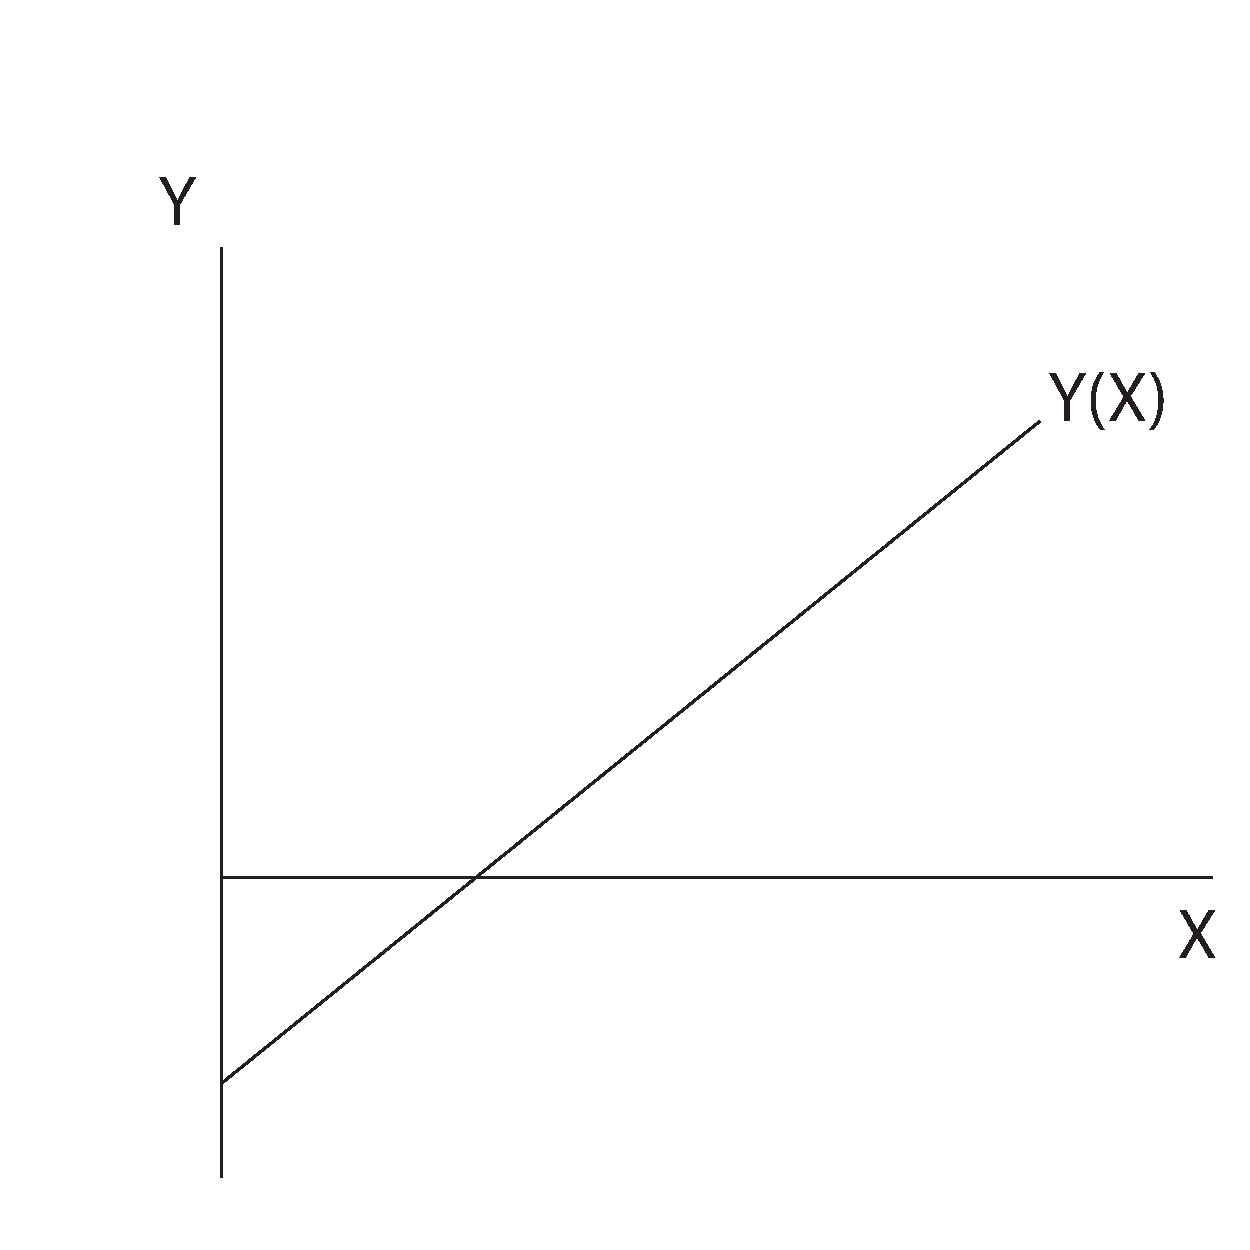
\includegraphics[width=200pt]{sample-figure}
  \end{center}
\end{frame}



\section{Conclusion}

\begin{frame}[t]\frametitle{Conclusion}
\framesubtitle{some subtitle}
    \begin{itemize}
      \item some items
      \item some items
      \item some items
      \item some items
      \item some items
      \item some items
   \end{itemize}

\end{frame}


\end{document}
